\documentclass{standalone}
\usepackage{tikz}
\usetikzlibrary{patterns, positioning}


\begin{document}
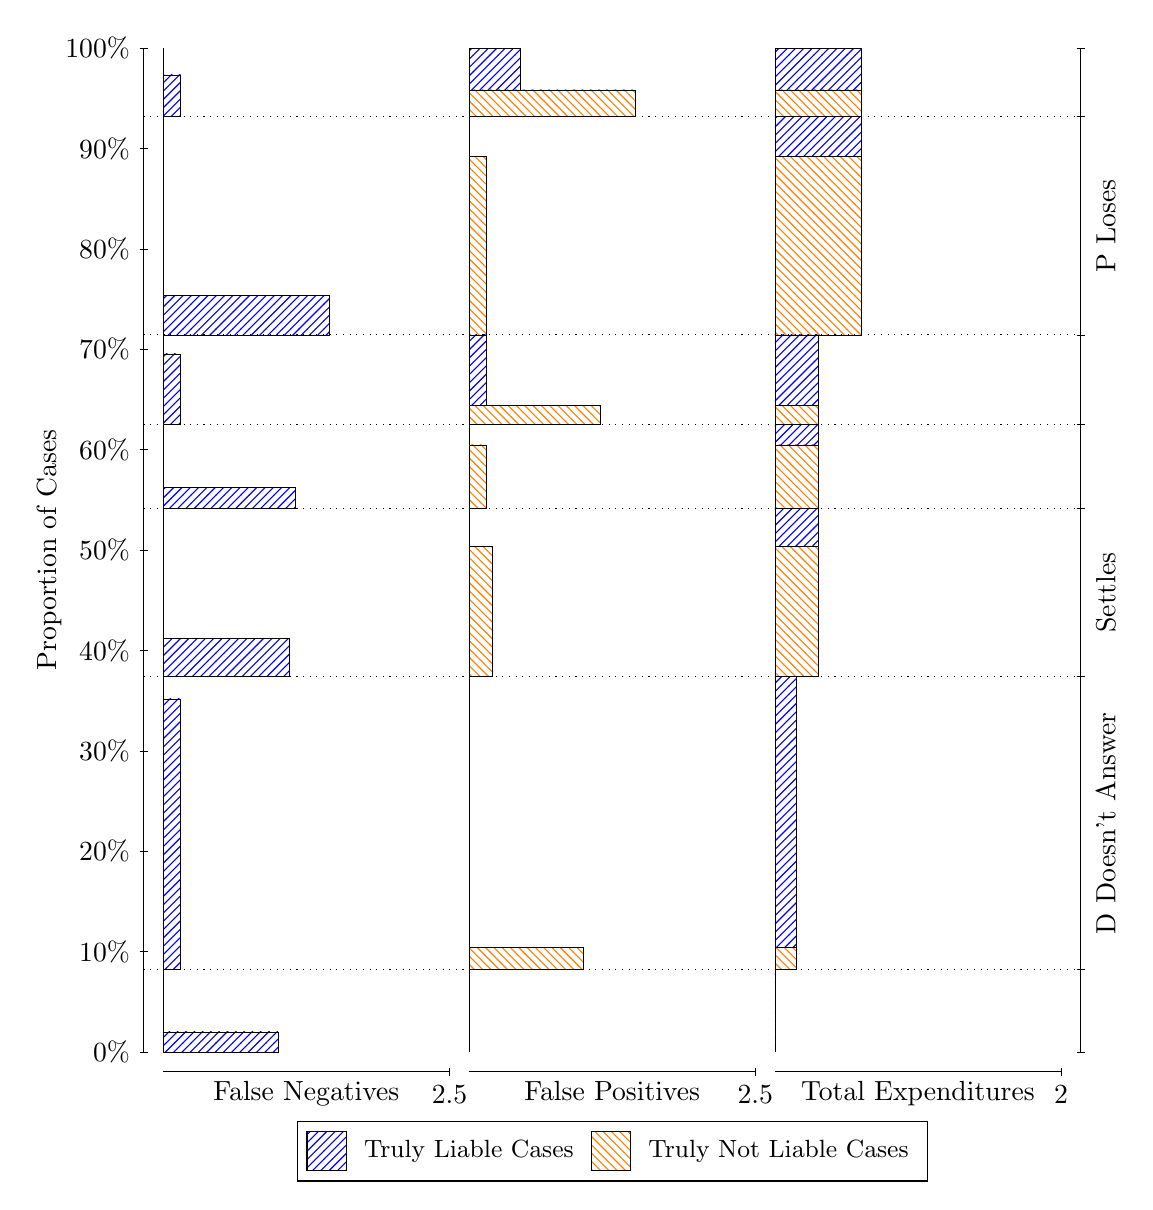
\begin{tikzpicture}
\draw[black, very thin] (1.5,1.75) -- (1.5,14.5);
\node[rotate=90, text=black, anchor=center] at (0.3, 8.125) {Proportion of Cases};
\draw[black, very thin] (1.45,1.75) -- (1.55,1.75);
\node[text=black, anchor=east] at (1.45, 1.75) {0\%};
\draw[black, very thin] (1.45,3.025) -- (1.55,3.025);
\node[text=black, anchor=east] at (1.45, 3.025) {10\%};
\draw[black, very thin] (1.45,4.3) -- (1.55,4.3);
\node[text=black, anchor=east] at (1.45, 4.3) {20\%};
\draw[black, very thin] (1.45,5.575) -- (1.55,5.575);
\node[text=black, anchor=east] at (1.45, 5.575) {30\%};
\draw[black, very thin] (1.45,6.85) -- (1.55,6.85);
\node[text=black, anchor=east] at (1.45, 6.85) {40\%};
\draw[black, very thin] (1.45,8.125) -- (1.55,8.125);
\node[text=black, anchor=east] at (1.45, 8.125) {50\%};
\draw[black, very thin] (1.45,9.4) -- (1.55,9.4);
\node[text=black, anchor=east] at (1.45, 9.4) {60\%};
\draw[black, very thin] (1.45,10.675) -- (1.55,10.675);
\node[text=black, anchor=east] at (1.45, 10.675) {70\%};
\draw[black, very thin] (1.45,11.95) -- (1.55,11.95);
\node[text=black, anchor=east] at (1.45, 11.95) {80\%};
\draw[black, very thin] (1.45,13.225) -- (1.55,13.225);
\node[text=black, anchor=east] at (1.45, 13.225) {90\%};
\draw[black, very thin] (1.45,14.5) -- (1.55,14.5);
\node[text=black, anchor=east] at (1.45, 14.5) {100\%};

\draw[black, very thin] (13.4,1.75) -- (13.4,14.5);
\draw[black, very thin] (13.35,1.75) -- (13.45,1.75);
\node[anchor=west] at (13.35, 1.75) {};
\draw[black, very thin] (13.35,2.7958) -- (13.45,2.7958);
\node[anchor=west] at (13.35, 2.7958) {};
\draw[black, very thin] (13.35,6.5159) -- (13.45,6.5159);
\node[anchor=west] at (13.35, 6.5159) {};
\draw[black, very thin] (13.35,8.6568) -- (13.45,8.6568);
\node[anchor=west] at (13.35, 8.6568) {};
\draw[black, very thin] (13.35,9.7214) -- (13.45,9.7214);
\node[anchor=west] at (13.35, 9.7214) {};
\draw[black, very thin] (13.35,10.857) -- (13.45,10.857);
\node[anchor=west] at (13.35, 10.857) {};
\draw[black, very thin] (13.35,13.628) -- (13.45,13.628);
\node[anchor=west] at (13.35, 13.628) {};
\draw[black, very thin] (13.35,14.5) -- (13.45,14.5);
\node[anchor=west] at (13.35, 14.5) {};

\draw[black, very thin, pattern color=blue, pattern=north east lines] (1.75,1.75) rectangle (3.2033,2.0064);
\draw[black, very thin, pattern color=orange, pattern=north west lines] (1.75,2.0064) rectangle (1.75,2.7958);
\draw[black, very thin, pattern color=blue, pattern=north east lines] (1.75,2.7958) rectangle (1.968,6.2355);
\draw[black, very thin, pattern color=orange, pattern=north west lines] (1.75,6.2355) rectangle (1.75,6.5159);
\draw[black, very thin, pattern color=blue, pattern=north east lines] (1.75,6.5159) rectangle (3.3487,7.0033);
\draw[black, very thin, pattern color=orange, pattern=north west lines] (1.75,7.0033) rectangle (1.75,8.6568);
\draw[black, very thin, pattern color=blue, pattern=north east lines] (1.75,8.6568) rectangle (3.4213,8.9171);
\draw[black, very thin, pattern color=orange, pattern=north west lines] (1.75,8.9171) rectangle (1.75,9.7214);
\draw[black, very thin, pattern color=blue, pattern=north east lines] (1.75,9.7214) rectangle (1.968,10.615);
\draw[black, very thin, pattern color=orange, pattern=north west lines] (1.75,10.615) rectangle (1.75,10.857);
\draw[black, very thin, pattern color=blue, pattern=north east lines] (1.75,10.857) rectangle (3.8573,11.362);
\draw[black, very thin, pattern color=orange, pattern=north west lines] (1.75,11.362) rectangle (1.75,13.628);
\draw[black, very thin, pattern color=blue, pattern=north east lines] (1.75,13.628) rectangle (1.968,14.16);
\draw[black, very thin, pattern color=orange, pattern=north west lines] (1.75,14.16) rectangle (1.75,14.5);
\draw[black, very thin, pattern color=orange, pattern=north west lines] (5.6333,1.75) rectangle (5.6333,2.5394);
\draw[black, very thin, pattern color=blue, pattern=north east lines] (5.6333,2.5394) rectangle (5.6333,2.7958);
\draw[black, very thin, pattern color=orange, pattern=north west lines] (5.6333,2.7958) rectangle (7.0867,3.0762);
\draw[black, very thin, pattern color=blue, pattern=north east lines] (5.6333,3.0762) rectangle (5.6333,6.5159);
\draw[black, very thin, pattern color=orange, pattern=north west lines] (5.6333,6.5159) rectangle (5.924,8.1695);
\draw[black, very thin, pattern color=blue, pattern=north east lines] (5.6333,8.1695) rectangle (5.6333,8.6568);
\draw[black, very thin, pattern color=orange, pattern=north west lines] (5.6333,8.6568) rectangle (5.8513,9.4611);
\draw[black, very thin, pattern color=blue, pattern=north east lines] (5.6333,9.4611) rectangle (5.6333,9.7214);
\draw[black, very thin, pattern color=orange, pattern=north west lines] (5.6333,9.7214) rectangle (7.3047,9.963);
\draw[black, very thin, pattern color=blue, pattern=north east lines] (5.6333,9.963) rectangle (5.8513,10.857);
\draw[black, very thin, pattern color=orange, pattern=north west lines] (5.6333,10.857) rectangle (5.8513,13.122);
\draw[black, very thin, pattern color=blue, pattern=north east lines] (5.6333,13.122) rectangle (5.6333,13.628);
\draw[black, very thin, pattern color=orange, pattern=north west lines] (5.6333,13.628) rectangle (7.7407,13.968);
\draw[black, very thin, pattern color=blue, pattern=north east lines] (5.6333,13.968) rectangle (6.2873,14.5);
\draw[black, very thin, pattern color=orange, pattern=north west lines] (9.5167,1.75) rectangle (9.5167,2.5394);
\draw[black, very thin, pattern color=blue, pattern=north east lines] (9.5167,2.5394) rectangle (9.5167,2.7958);
\draw[black, very thin, pattern color=orange, pattern=north west lines] (9.5167,2.7958) rectangle (9.7892,3.0762);
\draw[black, very thin, pattern color=blue, pattern=north east lines] (9.5167,3.0762) rectangle (9.7892,6.5159);
\draw[black, very thin, pattern color=orange, pattern=north west lines] (9.5167,6.5159) rectangle (10.062,8.1695);
\draw[black, very thin, pattern color=blue, pattern=north east lines] (9.5167,8.1695) rectangle (10.062,8.6568);
\draw[black, very thin, pattern color=orange, pattern=north west lines] (9.5167,8.6568) rectangle (10.062,9.4611);
\draw[black, very thin, pattern color=blue, pattern=north east lines] (9.5167,9.4611) rectangle (10.062,9.7214);
\draw[black, very thin, pattern color=orange, pattern=north west lines] (9.5167,9.7214) rectangle (10.062,9.963);
\draw[black, very thin, pattern color=blue, pattern=north east lines] (9.5167,9.963) rectangle (10.062,10.857);
\draw[black, very thin, pattern color=orange, pattern=north west lines] (9.5167,10.857) rectangle (10.607,13.122);
\draw[black, very thin, pattern color=blue, pattern=north east lines] (9.5167,13.122) rectangle (10.607,13.628);
\draw[black, very thin, pattern color=orange, pattern=north west lines] (9.5167,13.628) rectangle (10.607,13.968);
\draw[black, very thin, pattern color=blue, pattern=north east lines] (9.5167,13.968) rectangle (10.607,14.5);
\draw[black, dotted] (1.5,2.7958) -- (13.4,2.7958);
\draw[black, dotted] (1.5,6.5159) -- (13.4,6.5159);
\draw[black, dotted] (1.5,8.6568) -- (13.4,8.6568);
\draw[black, dotted] (1.5,9.7214) -- (13.4,9.7214);
\draw[black, dotted] (1.5,10.857) -- (13.4,10.857);
\draw[black, dotted] (1.5,13.628) -- (13.4,13.628);
\draw[black, very thin] (1.75,1.5) -- (5.3833,1.5);
\node[text=black, anchor=north] at (3.5667, 1.5) {False Negatives};
\draw[black, very thin] (5.3833,1.45) -- (5.3833,1.55);
\node[text=black, anchor=north] at (5.3833, 1.45) {2.5};

\draw[black, very thin] (5.6333,1.5) -- (9.2667,1.5);
\node[text=black, anchor=north] at (7.45, 1.5) {False Positives};
\draw[black, very thin] (9.2667,1.45) -- (9.2667,1.55);
\node[text=black, anchor=north] at (9.2667, 1.45) {2.5};

\draw[black, very thin] (9.5167,1.5) -- (13.15,1.5);
\node[text=black, anchor=north] at (11.333, 1.5) {Total Expenditures};
\draw[black, very thin] (13.15,1.45) -- (13.15,1.55);
\node[text=black, anchor=north] at (13.15, 1.45) {2};


\node[text=black, centered, rotate=90] at (13.72, 4.6558) {D Doesn't Answer};
\node[text=black, centered, rotate=90] at (13.72, 7.5864) {Settles};


\node[text=black, centered, rotate=90] at (13.72, 12.242) {P Loses};


\draw (7.449999999999999,1.5) node[draw=none] (baseCoordinate) {};
\begin{scope}[align=center]
        \matrix[scale=0.5, draw=black, below=0.5cm of baseCoordinate, nodes={draw}, column sep=0.1cm]{
            \node[rectangle, draw, minimum width=0.5cm, minimum height=0.5cm, pattern color=blue, pattern=north east lines] {}; &
            \node[draw=none, font=\small, text=black] (B) {Truly Liable Cases}; &
            \node[rectangle, draw, minimum width=0.5cm, minimum height=0.5cm, pattern color=orange, pattern=north west lines] {}; &
            \node[draw=none, font=\small, text=black] (B) {Truly Not Liable Cases}; \\
            };
\end{scope}

\end{tikzpicture}
\end{document}